\chapter{Concurrent Datatypes}
\label{chap:datatypes}

A \emph{concurrent datatype} is a datatype, for example, a queue, stack, set
or mapping, that can be safely accessed concurrently by multiple threads.
Operation invocations should appear to take place in a one-at-a-time order,
without interference.

Threads that use the concurrent datatype can act much as they would with a
sequential datatype: the implementer of the threads does not need to think
much about concurrency.  

The implementer of the concurrent datatype \emph{does} have to think about
concurrency, and ensure different operation calls do not interfere with one
another.  But that concurrency is local, often inside a single object: local
reasoning is much easier than global reasoning.  And there's a lot of scope
for re-using concurrent datatypes.

Datatype-based concurrent programming encapsulates \emph{all} the concurrency
within a small number of concurrent datatypes.

%%%%%%%%%%%%%%%%%%%%%%%%%%%%%%%%%%%%%%%%%%%%%%%%%%%%%%%%%%%%

\section{Example: a concurrent queue}
\label{sec:total-queue}

To illustrate some of the ideas, we will implement a concurrent queue.  First,
we should ask: what interface should a concurrent queue have?  A sequential
queue would typically have an interface like:
%
\begin{mysamepage}
\begin{scala}
trait Queue[T]{
  /** Enqueue x. */
  def enqueue(x: T): Unit

  /** Dequeue a value.  Precondition: the queue is not empty. */
  def dequeue(): T

  /** Is the queue empty? */
  def isEmpty: Boolean
}
\end{scala}
\end{mysamepage}
%
The |dequeue| operation has a non-trivial precondition, so client code that
uses the queue would be expected to check this first, for example, via code
such as:
\begin{scala}
  if(queue.isEmpty){ ... /* Handle the empty queue. */ } 
  else{ val x = queue.dequeue(); ... /* Do something with £x£. */ }
\end{scala}

However, this won't work with multi-threaded code: thread~$t$ might check that
the queue is non-empty; but then other threads might empty the queue before
$t$ attempts the |dequeue|, at which point the precondition is violated.  This
is a time-of-check to time-of-use (TOCTTOU) problem: there is a delay between
the thread checking the relevant precondition and performing the operation that
depends upon it, during  which the precondition becomes false; several
exercises in Chapter~\ref{chap:intro} considered the same issue.

We saw in Chapter~\ref{chap:clientServer} that there are two main ways of
dealing with operations that have a non-trivial precondition.  One way is to
return a special value to indicate that the precondition does not hold.  In
Scala, it is natural to use an |Option| value, with |None| indicating that the
precondition does not hold.  In some circumstances, it might be appropriate
(and more efficient) to use |null| for this, if |null| can never be returned
when the precondition does hold.  An alternative, is for the operation to
throw an exception, and expect the thread to catch it.  Operations that treat
preconditions in this way are called \emph{total}: they can take effect in any
state.

The other way to deal with the case that the precondition does not hold is to
block the thread until the precondition becomes true.  Such operations are
called \emph{partial}.

We will start with a total concurrent queue, with the following interface,
where the |dequeue| operation returns an |Option| type, with |None| used to
indicate am empty queue. 
%
\begin{mysamepage}
\begin{scala}
/** A total queue. */
trait TotalQueue[T]{
  /** Enqueue x. */
  def enqueue(x: T): Unit

  /** Dequeue a value.  Returns £None£ if the queue is empty. */
  def dequeue(): Option[T]

  /** Shut down the queue. */
  def shutdown: Unit
}
\end{scala}
\end{mysamepage}

A thread that performs a |dequeue| should handle both cases, for example, via
code such as:
\begin{scala}
  queue.dequeue() match{
    case Some(x) => ... // Do something with £x£.
    case None => ... // Handle the empty queue.
  }
\end{scala}

Figure~\ref{fig:total-queue-server} gives a straightforward implementation of
a total queue that encapsulates a server.  But we could also implement the
queue using one of the techniques we'll see later in the course.  The server
stores the queue itself (using a |Queue| from the Scala API).  Clients use
channels to cause the server to enqueue and dequeue values.  Note that the
server handles operations in a one-at-a-time way, preventing operations from
interfering with one another.  We also include a |shutdown| operation, to
provide a way to terminate the server thread, and so allow garbage collection.

%%%%%

\begin{figure}
\begin{scala}
class ServerTotalQueue[T] extends TotalQueue[T]{
  // Channels used for enqueueing and dequeueing.
  private val enqueueChan = new SyncChan[T]
  private val dequeueChan = new SyncChan[Option[T]]

  def enqueue(x: T) = enqueueChan!x

  def dequeue(): Option[T] = dequeueChan?()

  private def server = thread("ServerTotalQueue"){
    val queue = new scala.collection.mutable.Queue[T]
    serve(
      enqueueChan =?=> { x => queue.enqueue(x) }
      | dequeueChan =!=> { 
          if(queue.nonEmpty) Some(queue.dequeue()) else None 
        }
    )
  }

  fork(server)

  def shutdown() = { enqueueChan.close; dequeueChan.close }
\end{scala}
\caption{A total queue implemented using a server.}
\label{fig:total-queue-server}
\end{figure}

%%%%%

\begin{instruction}
Study the details of the implementation.
\end{instruction}


 % concurrent total queue, using a server;
\section{Linearization: Correctness of Concurrent Datatypes}
\label{sec:linearization}

We want to test the concurrent total queue implementation.  But first, we need
to understand better what ``correct'' actually means in this case.  And, by
extension, we will understand correctness conditions for other concurrent
datatypes. 

We define a \emph{history} to be a sequence of calls and returns of
operations, corresponding to threads operating on the datatype.
Informally, a history is correct if:
%
\begin{itemize}
\item Operation executions take place (apparently) in a one-at-a-time
  way, without interference between different executions.

\item The point at which each operation execution takes effect is between the
time the invocation was invoked and when it returns; we call this point
the \emph{linearization point}.

\item The values returned by operation executions should be the same as for a
sequential queue (when the executions are performed in the same order).
\end{itemize}
%
The correctness condition for other concurrent datatypes is the same, except
with the sequential queue in the third item replaced by a corresponding
sequential datatype.

This property is called \emph{linearization}~\cite{herlihy-wing}.  It is an
attractive property, because it matches most programmers' mental models of how
such a concurrent datatype should behave.

We will give a more formal definition of linearization shortly.  But first, we
give some examples.  

Figure~\ref{fig:linearization} gives four timelines depicting histories.  In
each timeline, time goes from left to right.  Each row is labelled with the
identity of a thread (e.g.~$t_0$).  Each horizontal line represents the
execution of an operation, with the endpoints of the line representing the
call of the operation and its return, respectively; the line is labelled with
the name of the operation, its parameters, and the value returned, although we
omit the latter for operations, like |enqueue|, that return the trivial |Unit|
type.

%%%%%

\begin{figure}
\def\X{node{\scalastyle X};}
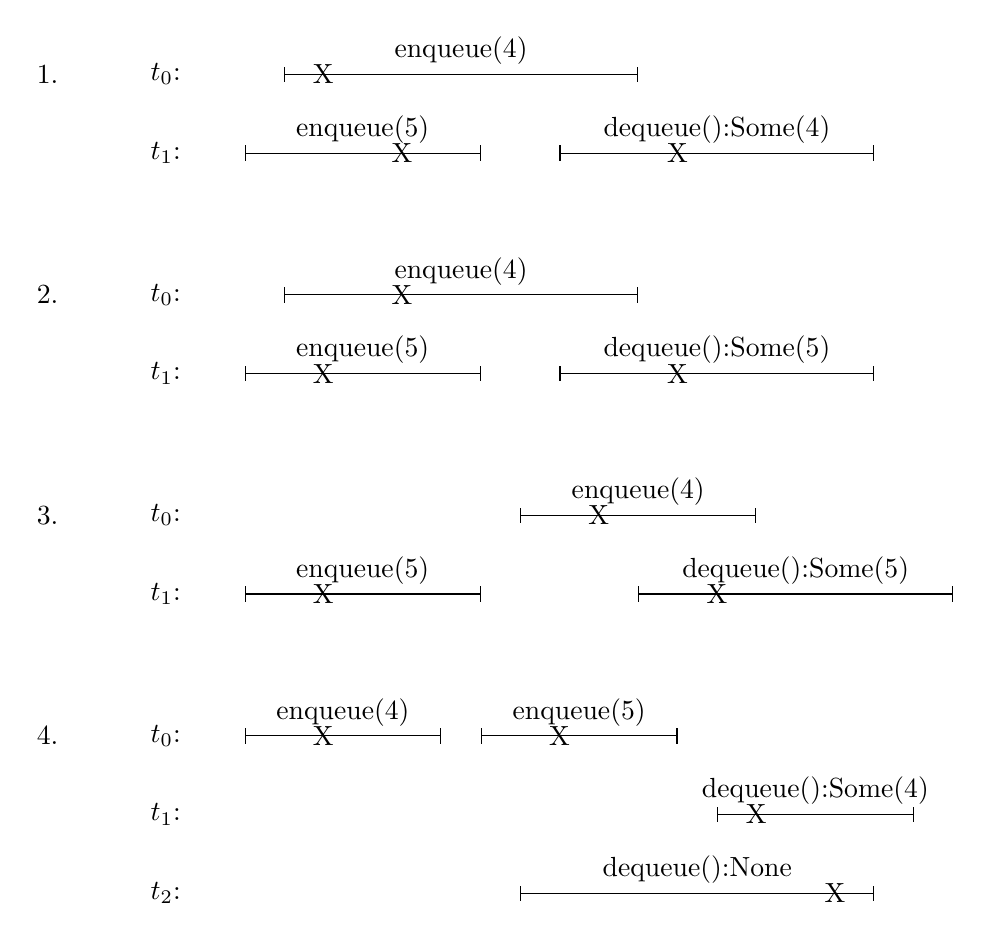
\begin{tikzpicture}[scale=1.0]
\draw (-1.5,0) node{1.};
\draw (0,0) node {$t_0$:}; 
\draw[|-|] (1.5,0) -- node[above] {\scalashape enqueue(4)} (6,0);
\draw(2,0) \X;
\draw (0,-1) node {$t_1$:}; 
\draw[|-|] (1,-1) -- node[above] {\scalashape enqueue(5)} (4,-1);
\draw(3,-1) \X;
\draw[|-|] (5,-1) -- node[above] {\scalashape dequeue():Some(4)} (9,-1);
\draw(6.5,-1) \X;
%%%%%
\draw (0,-2.8) node (O) {$t_0$:}; 
\draw (O)++(-1.5,0) node{2.};
\draw[|-|] (O)++(1.5,0) -- node[above] {\scalashape enqueue(4)} ++(4.5,0);
\draw (O)++(3,0) \X;
\draw (O)++(0,-1) node {$t_1$:}; 
\draw[|-|] (O)++(1,-1) -- node[above] {\scalashape enqueue(5)} ++(3,0);
\draw (O)++(2,-1) \X;
\draw[|-|] (O)++(5,-1) -- node[above] {\scalashape dequeue():Some(5)} ++(4,0);
\draw(O)++(6.5,-1) \X;
%%%%%
\draw (O)++(0,-2.8) node (O) {$t_0$:}; 
\draw (O)++(-1.5,0) node{3.};
\draw[|-|] (O)++(4.5,0) -- node[above] {\scalashape enqueue(4)} ++(3,0);
\draw (O)++(5.5,0) \X;
\draw (O)++(0,-1) node {$t_1$:}; 
\draw[|-|] (O)++(1,-1) -- node[above] {\scalashape enqueue(5)} ++(3,0);
\draw (O)++(2,-1) \X;
\draw[|-|] (O)++(6,-1) -- node[above] {\scalashape dequeue():Some(5)} ++(4,0);
\draw (O)++(7,-1) \X;
%%%%%
\draw (O)++(0,-2.8) node (O) {$t_0$:}; 
\draw (O)++(-1.5,0) node{4.};
\draw[|-|] (O)++(1,0) -- node[above] {\scalashape enqueue(4)} ++(2.5,0);
\draw (O)++(2,0) \X;
\draw[|-|] (O)++(4,0) -- node[above] {\scalashape enqueue(5)} ++(2.5,0);
\draw (O)++(5,0) \X;
\draw (O)++(0,-1) node{$t_1$:};
\draw[|-|] (O)++(7,-1) -- 
  node[above] {\scalashape dequeue():Some(4)} ++(2.5,0);
\draw (O)++(7.5,-1) \X;
\draw (O)++(0,-2) node{$t_2$:};
\draw[|-|] (O)++(4.5,-2) -- 
  node[above] {\scalashape dequeue():None} ++(4.5,0);
\draw (O)++(8.5,-2) \X;
\end{tikzpicture}
\caption{Four timelines illustrating linearization.}
\label{fig:linearization}
\end{figure}

%%%%%

In timeline~1, thread $t_0$ enqueues~|4|, and thread $t_1$ enqueues~|5| and
dequeues~|4| (so the |dequeue| operation returns |Some(4)|).  This history is
linearizable, if the operations take place at the linearization points
labelled~``{\scalashape X}''.  This would correspond to a sequential
history:\footnote{We denote sequences within angle brackets, $\seq{\ldots}$.}
\[\mstyle
\seq{ \sm{enqueue(4)},\, \sm{enqueue(5)},\, \sm{dequeue():Some(4)}}
\]
which would be valid on a corresponding sequential queue.

%%%%%

Timeline~2 is similar, except the |dequeue| returns |Some(5)|.  This history
is also linearizable, where the operations take place at the points
labelled~``{\scalashape X}'', which would correspond to the valid sequential
history
\[\mstyle
\seq{ \sm{enqueue(5)},\, \sm{enqueue(4)},\, \sm{dequeue():Some(5)}}
\]
In each of timelines~1 and~2, the two |enqueue|s overlap in time, which means
they could take place in either order: the subsequent |dequeue| reveals the
order. 

%%%%%

In timeline~3, the enqueue of~|5| returns before the enqueue of~|4| is
called.  That means that the two enqueues must take place in that order, since
each linearization point must be within the time period of the operation
execution.  The timeline is linearizable, as shown by the labelled
linearization points.  However, if the |dequeue| had returned |Some(4)|, the
history would not be linearizable. 

By contrast, timeline~4 is not linearizable: the |dequeue| by thread~$t_2$
should not return |None|, because the queue is nonempty throughout that
operation's execution.  For example, the illustrated linearization points
would correspond to the sequential history
\[\mstyle
\seq{ \sm{enqueue(4)},\, \sm{enqueue(5)},\,
   \sm{dequeue():Some(4)},\, \sm{dequeue():None}},
\]
which is invalid, since the second |dequeue| should return |Some(5)|.  An
alternative choice for the linearization points would correspond to the
sequential history 
\[\mstyle
\seq{ \sm{enqueue(4)},\, \sm{dequeue():None}},\, \sm{enqueue(5)},\,
   \sm{dequeue():Some(4)},
\]
which is again invalid.


It is important that we use \emph{synchronous channels} in the server-based
queue.  Suppose we had used buffered channels.  Then the following behaviour
is possible:
%
\begin{enumerate}
\item Thread $t_1$ calls |enqueue(5)|, but the value~|5| stays in the
  |enqueueChan|, even after $t_1$ returns;

\item Thread $t_2$ calls |dequeue()|, and the server sends it |None|.
\end{enumerate}
%
This history is not linearizable: it would necessarily correspond to the
sequential history
\[\mstyle
\seq{ \sm{enqueue(5)},\, \sm{dequeue():None}},
\]
which is not valid.
Alternatively:
%
\begin{enumerate}
\item The server sends |None| on |dequeueChan|, and that value stays in the
  channel; 

\item Thread $t_1$ calls |enqueue(5)|, this value is received and stored
  by the server, and $t_1$ returns;  

\item Thread $t_2$ calls |dequeue()|, and receives the |None| sent earlier.
\end{enumerate}
%
This history is not linearizable: it would again correspond to the previous
sequential history.

Using synchronous channels, the invocations have an effect in the order of the
channel communications.  This order is compatible with the order of the
invocations calls and returns.  We will always use synchronous channels when
implementing a concurrent datatype using a server thread.

%%%%%%%%%%

\subsection{Defining linearization}

We now give a formal definition of linearization, although nearly always the
earlier informal description is enough.  

A \emph{concurrent history} of an object~$o$ records the calls and returns of
operations on~$o$.  It is a sequence of events of the following forms:
%
\begin{itemize}
\item $\call.op^i(x)$, representing a call of operation~$op$ with
  parameter(s)~$x$;
\item $\return.op^i \:: y$, representing a return of an execution of~$op$,
  giving result~$y$.
\end{itemize}
%
Here $i$ is a \emph{execution identity}, used to identify a particular
execution, and to link the $\call$ and corresponding~$\return$.  For example,
timeline~1 in Figure~\ref{fig:linearization} represents the history
\[\mstyle
\langle
  \begin{align}
  \call.\enqueue^1\sm{(5)},\, \call.\enqueue^2\sm{(4)},\,
  \return.\enqueue^1\::\sm{()}, \\
  \quad \call.\dequeue^3\sm{()},\, \return.\enqueue^2\::\sm{()},\,
  \return.\dequeue^3\::\sm{Some(4)} \rangle .
  \end{align}
\]
(We normally represent histories by timelines, since they are much easier to
understand.)  In order to be well formed, each execution identity must appear
on at most one $\call$ event and at most one $\return$ event; and for each
event $\return.op^i\::y$, the history must contain an earlier event
$\call.op^i(x)$, i.e.~for the same operation and execution identity.  We
consider only well formed histories from now on.  
%% In examples, we will omit
%% return values of the unit value~|()| from |enqueue|s.

We say that a $\call$ event and a $\return$ event \emph{match}
if they have the same execution identifier.  A concurrent history is
\emph{complete} if for every $\call$ event, there is a matching $\return$
event, i.e.~no execution is still pending at the end of the history.  Each of
the histories depicted in Figure~\ref{fig:linearization} is complete. 

Linearisation is specified with respect to a sequential specification
object~$Spec$, with the same operations and signatures as the concurrent
object in question.  For the case of a total queue, we could define the
sequential specification object as follows:
%
\begin{scala}
class SeqQueue[T]{
  private val q = new scala.collection.mutable.Queue[T]

  def enqueue(x: T) = q.enqueue(x)

  def dequeue(): Option[T] = if(q.isEmpty) None else Some(q.dequeue())
}
\end{scala}
%
A history of the specification object is a sequence of events of the form:
%
\begin{itemize}
\item $op^i(x)\::y$ representing an execution of operation~$op$ with
  parameter~$x$, returning result~$y$; again $i$~is an execution identity,
  which must appear at most once in the history.
\end{itemize}
%
Such histories are designated as \emph{legal} if they are consistent with the
definition of~$Spec$.  Earlier, we gave several legal histories for |SeqQueue|
(although we omitted execution identities).

Let $h$ be a complete concurrent history, and let $h_s$ be a legal history of
the specification object.  We say that $h$ and~$h_s$ \emph{correspond} if they
contain the same executions, i.e., for each $\call.op^i(x)$ and
$\return.op^i\::y$ in $h$,\, $h_s$ contains $op^i(x)\::y$, and vice versa.  We
say that $h_s$ is a \emph{linearisation} of~$h$ if there is some way of
interleaving the two histories (i.e.~creating a history containing the events
of~$h$ and~$h_s$, preserving the order of events) such that each $op^i(x)\::y$
occurs between $\call.op^i(x)$ and $\return.op^i\::y$.  Informally, this
indicates that the executions of~$h$ appeared to take place in the order
described by~$h_s$, and that this order is legal according to the
specification object.

For example, the following is an interleaving of the complete concurrent
history and the legal sequential history corresponding to timeline~1 in
Figure~\ref{fig:linearization}: each event of the sequential history is
between the corresponding events of the concurrent history. 
\[\mstyle
\langle
  \begin{align}
  \call.\enqueue^1\sm{(5)},\, \call.\enqueue^2\sm{(4)},\,  
  \enqueue^2\sm{(4)}\::\sm{()},\,
  \enqueue^1\sm{(5)}\::\sm{()},\, \\
\quad
  \return.\enqueue^1\::\sm{()}, \,
  \call.\dequeue^3\sm{()},\, \return.\enqueue^2\::\sm{()},\, \\
\quad
  \dequeue^3\sm{()}\::\sm{Some(4)},\,
  \return.\dequeue^3\::\sm{Some(4)} \rangle .
  \end{align}
\]

A concurrent history might not be complete, i.e.~it might have some pending
executions that have been called but have not returned.  An \emph{extension}
of a concurrent history~$h$ is formed by adding zero or more $\return$ events
corresponding to pending executions.  We write $complete(h)$ for the
subsequence of~$h$ formed by removing all $\call$ events corresponding to
pending executions.

We say that a (not necessarily complete) concurrent history~$h$ is
\emph{linearisable} if there is an extension~$h'$ of~$h$ such that
$complete(h')$ is linearisable.  Informally, the $\return$ events that are
in~$h'$ but not~$h$ are for operation executions that have had an effect, but
not returned in~$h$; the $\call$ events removed in $complete(h')$ are for
operation executions that have not yet had an effect.

For example, consider the history
\begin{eqnarray*}
h & = & \langle
  \begin{align} 
  \call.\enqueue^1\sm{(5)},\, \call.\dequeue^2\sm{()},\, \\
  \quad  \call.\dequeue^3\sm{()},\,  \return.\dequeue^2\::\sm{Some(5)} \rangle.
  \end{align}
\end{eqnarray*}
This is incomplete because the |enqueue| and the dequeue with execution
identity~$3$ are both pending.  Consider the extension $h'$ formed by adding
$\return.\enqueue^1\::\sm{()}$ at the end.  Then $complete(h')$ is
\[\mstyle
\langle 
  \call.\enqueue^1\sm{(5)},\, \call.\dequeue^2\sm{()},\,
  \return.\dequeue^2\::\sm{Some(5)},\, \return.\enqueue^1\::\sm{()}\rangle,
\]
which is linearisable; hence $h$ is also linearisable.  In~$h$, the |enqueue|
has had an effect, so is included in $complete(h')$; but the latter |dequeue|
has not had an effect, so is omitted.

We say that a concurrent object is linearisable if all of its histories are
linearisable.


 % linearizability 
\section{Testing for Linearizability}

We now consider how we can test the implementation of a total concurrent queue
from Section~\ref{sec:total-queue}, and more generally, how we can test other
implementations of concurrent datatypes.

The basic idea is as follows. We run some threads on the concurrent datatype,
performing random operations, and record the history of operation calls and
returns.  We then search for a corresponding sequential history that explains
linearizability, and that is a valid history for the corresponding sequential
datatype.  If none is found, we signal an error.  We can repeat this procedure
many times.

Algorithms for searching for the corresponding sequential history have been
investigated by Wing and Gong~\cite{wing-gong}, and by
me~\cite{gavin:lin-testing}.  The SCL library includes the latter, which can
be used without understanding the underlying algorithms. 

Figure~\ref{fig:queue-lin-tester} gives a stripped-down testing script for a
concurrent total queue.  (The full version, on the book website, can be used
with multiple concurrent queue implementations, and replaces the numerical
constants by variables, specifiable via the command line.)

%%%%%

\begin{figure}
\begin{scala}[numbers = left]
object QueueTest{
  /* The concurrent datatype, and sequential specification type. */
  type ConcQueue = TotalQueue[Int] 
  type SeqQueue = scala.collection.immutable.Queue[Int]

  /* Sequential operations. */
  def seqEnqueue(x: Int)(q: S): (Unit, S) = ((), q.enqueue(x))£\label{line:seqEnqueue}£
  def seqDequeue(q: S): (Option[Int], S) =   
    if(q.isEmpty) (None, q) 
    else{ val (r,q1) = q.dequeue(); (Some(r), q1) }

  /** A worker in the testing system. */
  def worker(me: Int, log: LinearizabilityLog[S, C]) = {£\label{line:queue-lin-tester-worker}£
    val random = new scala.util.Random
    for(i <- 0 until 200)
      if(random.nextFloat() <= 0.3){
        val x = random.nextInt(20)
        log(_.enqueue(x), s"enqueue($x)", seqEnqueue(x))£\label{line:queue-lin-tester-worker-enqueue}£
      }
      else log(_.dequeue(), "dequeue", seqDequeue)£\label{line:queue-lin-tester-worker-dequeue}£
  }

  /** Perform a single test. */
  def doTest = {
    val concQueue = new ServerTotalQueue[Int]; val seqQueue = Queue[Int]()
    val tester = 
      LinearizabilityTester[SeqQueue,ConcQueue](seqQueue, concQueue, 4, worker)£\label{line:construct-lin-tester}£
    if(tester() <= 0) sys.exit()
    concQueue.shutdown()
  }

  def main(args: Array[String]) = {
    for(r <- 0 until 10000){ doTest; if(r%20 == 0) print(".") }
    println()
  }
}
\end{scala}
\caption{A linearizability tester for a concurrent total queue.}
\label{fig:queue-lin-tester}
\end{figure}

%%%%%

The test program works on a |TotalQueue[Int]|; we define |ConcQueue| as a type
synonym.

The test program also requires a corresponding sequential specification
object.  The underlying linearizability framework requires this to be
\emph{immutable} (unlike in Section~\ref{sec:linearization}): the state of the
specification object should not change; instead, operations produce new
instances of the same type.  The framework also requires the specification
object to be deterministic.  Here, we use an immutable queue
from the Scala API; we define |SeqQueue| as a type synonym. 

In general, given a type |S| of the sequential specification object, for each
operation |op: A| on the concurrent datatype, we need a corresponding function
|seqOp: S => (A, S)| on the sequential datatype, which returns the expected
value\footnote{More precisely, the two values should be equal, as tested using
  the ``{\scalashape ==}'' method.} (of type~|A|), paired with the new value
of the sequential datatype. 

For the case of a concurrent total queue, the relevant definitions are from
line~\ref{line:seqEnqueue}.  These are simple wrappers around the API
operations.  The operation |seqEnqueue(x)| corresponds to |enqueue(x)| on the
concurrent queue.  Given a sequential queue~|q|, this returns the unit value
(matching the return from~|enqueue|) and a new sequential queue, formed by
enqueuing~|x| on~|q|.  The operation |seqDequeue| corresponds to |dequeue()|
on the concurrent queue.  When given an empty queue~|q|, it returns |None| (to
match the value expected from |dequeue()|), and the original state of~|q|.
When given a nonempty queue, it performs a dequeue using the API
operation, which returns the value~|r| dequeued and the new state of the
queue, and then constructs the appropriate result (including |Some(r)|, to
match the value expected from |dequeue()|).

%%%%%

The function |worker| (from line~\ref{line:queue-lin-tester-worker}) defines
a worker that performs and logs operations on the concurrent datatype,
associating each concurrent operation with a corresponding operation on the
sequential datatype.  Here, the worker performs 200 operations; each is (with
probability 0.3) an enqueue of a random value, or (with probability~0.7) a
dequeue.


The worker takes a log object |log| as a parameter; each operation is
performed and logged via a call to |log| (more precisely, the |apply| function
of~|log|; see Scala box~\ref{sb:apply}), taking three parameters:
%
\begin{itemize}
\item
The operation to be performed on the concurrent datatype;

\item A string describing the operation: this is used in debugging output in
  the case that a non-linearizable history is found, and is also used
  internally for optimisations; semantically different operations should have
  distinct strings;

\item
The corresponding function on the sequential datatype.
\end{itemize}
%
The call to |log| logs the invocation of the concurrent operation,
performs the concurrent operation, and logs the result returned.

In Figure~\ref{fig:queue-lin-tester},
line~\ref{line:queue-lin-tester-worker-enqueue} performs |enqueue(x)| on the
concurrent queue, and associates it with the function |seqEnqueue(x)| on the
specification object.  Line~\ref{line:queue-lin-tester-worker-dequeue}
performs |dequeue()| on the concurrent queue, and associates it with the
function |seqDequeue| on the specification object.  Each uses an anonymous
function (see Scala box~\ref{sb:anon-function}) to define the operation on the
concurrent queue: each underscore (``\SCALA{_}'') represents a hole into which
the concurrent queue is placed.

The function |doTest| performs a single test.  This starts by creating a
concurrent queue to test, and a corresponding sequential specification object.
Line~\ref{line:construct-lin-tester} constructs a linearizability testing
object~|tester|.  This takes two type parameters, representing the type of
sequential specification objects and concurrent objects (we could omit these
type parameters, but I find it useful to include them).  It takes value
parameters representing the specification object, the concurrent object to be
tested, the number of worker threads to run (here~4), and the definition of a
worker.
%
The expression |tester()| then runs the testing object (by calling its |apply|
function).  This runs the workers concurrently, logging the operation calls on
the concurrent datatype.  It then tests whether the resulting history is
linearizable, returning a positive result if so, and otherwise printing
suitable debugging information on the screen.  The |doTest| function
terminates the program if the history is not linearizable.  Finally, it shuts
down the concurrent queue.

The |main| function calls |doTest| many times. 

Figure~\ref{fig:lin-testing-error} gives sample debugging information for a
(deliberately) incorrect implementation of a |TotalQueue|.  More precisely,
the implementation uses buffered channels, rather than synchronous channels;
we saw earlier why this is incorrect.  The test was run with just three worker
threads, each performing a single operation, so as to keep the history short.
The error is reflected by the value of |None| returned (at line~5) by the
|dequeue| done by thread~|2|.  Each of threads~|0| and~|1| had completed an
|enqueue| by this point, so the |dequeue| should have returned one of their
values; in fact, the |enqueue|s were concurrent, so could have been linearized
in either order, and so either of their values would have been allowed.

%%%%%  

\begin{figure}
\begin{verbatim}
0: 0 invokes enqueue(69)
1: 1 invokes enqueue(60)
2: 0 returns ()
3: 1 returns ()
4: 2 invokes dequeue
5: 2 returns None
-- Previous event not linearized
-- Allowed return values: Some(69), Some(60)
\end{verbatim}
\caption{Output of {\scalashape QueueTest} on a non-linearizable history.}
\label{fig:lin-testing-error}
\end{figure}

%%%%%

Linearizability testers for other concurrent datatypes take a very similar
form.  My normal approach to writing such a tester is to take an existing one
and to adapt it.  

Under the bonnet, the linearizability tester performs a search, in effect,
considers all possible linearizations of the history---i.e.~all ways of
ordering the operations consistent with the history---and testing whether that
ordering is compatible with the sequential datatype.  The search can complete
quite quickly in practice; for example, the tester in
Figure~\ref{fig:queue-lin-tester}, which performs 10,000 tests, with a total
of 8,000,000 operation executions, takes slightly more than two minutes to run
on my computer.

However, the search to linearize a particular history can be very large, and
so be time-consuming.  Indeed, the problem of deciding whether a given history
is linearizable is NP-complete in general, so there are bound to be some bad
cases.  It is therefore worth taking steps to limit the time taken by the
search.  A good pragmatic approach is to start with short runs---a small
number of threads performing a small number of operations each---and to move
to longer runs if the testing goes well.

Testing certain concurrent datatypes requires particular considerations.  In
the case of a queue, if two |enqueue|s happen concurrently, they could be
linearized in either order; the linearizability tester has to consider both
possibilities; which one is correct becomes apparent only when one of the
values is dequeued.  If the queue holds quite a lot of values, there might be
several pairs that were enqueued concurrently.  This means that the search
space can grow exponentially with the length of the queue.  To avoid this, we
should take steps to make it unlikely that the queue holds too many values.
In Figure~\ref{fig:queue-lin-tester}, we did this by making dequeues more
frequent than enqueues.

By default, the linearizability tester logs operation calls and returns using
thread-local logs, pairing each event with a timestamp.  We saw a similar
technique in an earlier chapter.  If you're using an operating system that
doesn't support timestamps property, setting the optional parameter |tsLog| to
|false| will use a different type of log; for example:
%
\begin{scala}
  val tester = LinearizabilityTester[SeqQueue, ConcQueue](
    seqQueue, concQueue, 4, worker, tsLog = false)
\end{scala}

It is worth reiterating that the sequential specification object must be
immutable: its state should not change.  Failing to respect this requirement
is a fairly common error.

It is beneficial to ensure that the specification object has a natural
definition for equality, and an associated hash code.  This is true for the
immutable |Queue|s we used here: two such objects are equal if they contain
the same sequence of data; and in this case their hash codes will be equal.
The same is true for other objects in the |scala.collection.immutable|
package.  The linearization checker uses a hash set to keep track of nodes of
the search graph it has seen previously, so as to avoid repeating work.  For
this to be effective, it needs to be able to identify when two sequential
specification objects represent the same state.

It is also worth reiterating that the strings used in logging semantically
different operations should be distinct.  My normal style is to use a string
that looks like the syntax of the operation call, including any parameters:
this is what is most useful in debugging output (if an error of
linearizability is found).  But also these strings are used internally as an
optimisation (the tester records the effect of each sequential operation on the
specification object, using the string as a key; this avoids repeating the
same operation on the same specification object).

 % linearizability testing


\begin{slide}
\heading{A partial queue}

In the previous chapter we implemented a total concurrent queue that returns
|None| if |dequeue| is called when the queue is empty.  
%
An alternative is to block that thread until there is a value to be dequeued.
This gives a partial queue, with the following interface.

\begin{scala}
trait PartialQueue[T]{
  /** Enqueue x. */
  def enqueue(x: T): Unit

  /** Dequeue a value.  Blocks until the queue is non-empty. */
  def dequeue(): T

  /** Shut down the queue. */
  def shutdown
}
\end{scala}
Note that if the queue is empty and all threads are attempting a dequeue, the
system will deadlock. 
\end{slide}

%%%%%

\begin{slide}
\heading{A partial queue}

\begin{scala}
class ServerPartialQueue[T] extends PartialQueue[T]{
  // Channel for dequeueing
  private val dequeueChan = new SyncChan[T]

  def dequeue(): T = dequeueChan?()

  private def server = thread{
    val queue = new scala.collection.mutable.Queue[T]
    serve(
      enqueueChan =?=> { x => queue.enqueue(x) }
      | queue.nonEmpty && dequeueChan =!=> queue.dequeue()
    )
  }

  ... // other parts as earlier
}
\end{scala}
\end{slide}

%%%%%

\begin{slide}
\heading{Testing}

We can test this queue for linearizability, much as for the previous version.
However, we have to amend the sequential specification object to recognise
that a dequeue cannot happen when the queue is empty. 
\begin{scala}
  def seqDequeue(q: S) : (Int, S) = {
    require(q.nonEmpty); q.dequeue()
  }
\end{scala}
An operation invocation on the concurrent datatype cannot be linearized in a
state where the corresponding operation on the sequential datatype throws an
|IllegalArgumentException|.

Also we have to be careful that we never get into a deadlocked state where all
the threads are attempting a dequeue from the empty queue.  I arrange for half
the threads to perform just enqueues, and the others to perform just dequeues.  
\end{slide}

%%%%%

\begin{slide}
\heading{Termination}

Suppose the queue is empty, and all the threads are attempting a dequeue.
With the previous design, the system would be deadlocked.

A better approach would be for the server to detect such a state, and react
accordingly.  We choose to shut down the queue in this case, and arrange for
each dequeue attempt to throw a |Stopped| exception (an alternative would be
to use an |Option| value).

In order to do this, the server needs to know how many threads are attempting
a dequeue.  That means we can't just block the |dequeueChan| channel when the
queue is empty.  Instead, we arrange for the dequeueing thread to pass a reply
channel on the |dequeueChan|.  These reply channels are stored until the
request can be made.  If the number of stored reply channels equals the number
of workers, the queue shuts down.
\end{slide}

%%%%%

\begin{slide}
\heading{Termination}

\begin{scala}
/** A partial queue that terminates if all worker threads are attempting to
  * dequeue, and the queue is empty.
  * @param numWorkers the number of worker threads. */
class TerminatingPartialQueue[A](numWorkers: Int){
  private type ReplyChan = Chan[A]
  /** Channel for dequeueing. */
  private val dequeueChan = new SyncChan[ReplyChan]

  /** Attempt to dequeue a value.
    * @throws Stopped exception if the queue has been shutdown. */
  def dequeue(): A = {
    val reply = new SyncChan[A] // or a BuffChan[A]
    dequeueChan!reply
    reply?()
  }
  ... 
}
\end{scala}
\end{slide}

%%%%%

\begin{slide}
\heading{Termination}

We might also want to externally shut down the server, (e.g.~in a search
algorithm, if we find what we're looking for).

It's necessary for the server to control termination in this case, so we
arrange for the |shutdown| method to send a message to the server. 
%
\begin{scala}
  private val shutdownChan = new SyncChan[Unit]

  /** Shut down this queue. */
  def shutdown = attempt{ shutdownChan!(()) }{ }
\end{scala}
Note: it's possible that the server has already terminated and |shutdownChan|
closed, in which case we catch the |Stopped| exception.

%% The construct
%% \begin{scala}
%%   attempt{ p }{ q }
%% \end{scala}
%% Executes |p|; but if |p| throws a |Stopped| exception, that exception is
%% caught, and |q| is executed. 
\end{slide}
  
%%%%%

\begin{slide}
\heading{The server}

\begin{scala}
  private def server = thread("server"){
    // Currently held values
    val queue = new Queue[A]()
    // Queue holding reply channels for current dequeue attempts.
    val waiters = new Queue[ReplyChan]()
    // Invariant: queue.isEmpty or waiters.isEmpty

    // Termination: signal to all waiting workers
    def close = {
      for(c <- waiters) c.close
      enqueueChan.close; dequeueChan.close; shutdownChan.close
    }
    ...
  }
\end{scala}
\end{slide}

%%%%%

\begin{slide}
\heading{The server main loop}

\begin{scala}
    serve(
      enqueueChan =?=> { x => 
        if(waiters.nonEmpty){ // pass x directly to a waiting dequeue
          assert(queue.isEmpty); waiters.dequeue()!x
        }
        else queue.enqueue(x)
      }
      | dequeueChan =?=> { reply =>
          if(queue.nonEmpty) reply!(queue.dequeue()) // service request immediately
          else{                                        // thread has to wait
            waiters.enqueue(reply)
            if(waiters.length == numWorkers) close
          }
        }
      | shutdownChan =?=> { _ => close }
    )
\end{scala}
\end{slide}
 % partial queue, including termination

\section{Example: graph search}

Many Computer Science applications involve searching in a graph (whether
explicitly or implicitly).  Examples include:
%
\begin{itemize}
\item Route planning, where the nodes of the graph are places, and the edges
  are roads between them;

\item Planning, where the nodes of the graph are intermediate stages towards
  some goal, and the edges are possible steps;

\item Puzzle solving, such as sudoku, where the nodes of the graph are partial
  solutions to the puzzle, and the edges correspond to steps of the puzzle;

\item Verification of some computer system, where the nodes of the graph are
  states that the system can reach, and the edges are transitions that the
  system can perform.  
\end{itemize}
%
Searches might aim to minimise some cost, or might aim to find a node with a
particular property.  Searches might use breadth-first search, depth-first
search, or some more specialised search algorithm such as Dijkstra's Algorithm
or the A$^*$ Algorithm.

In this section we will examine a concurrent algorithm to search a graph for a
node with a particular property, using approximate breadth-first search.
Exercise~\ref{ex:dfs} asks you to implement approximate concurrent
depth-first search.

We define a graph as an implementation of the trait |Graph[N]| in
Figure~\ref{fig:graph}.  The type parameter~|N| represents nodes.  The
function |succs(n)| gives the successors of node~|n|, i.e.~all nodes |n'| such
that there is an edge from |n| to |n'|.

%%%%%

\begin{figure}
\begin{scala}
/** A trait representing an unlabelled graph with nodes of type £N£. */
trait Graph[N]{
  /** The successors of node £n£. */
  def succs(n: N): List[N]
}

/** A trait representing a graph search problem in graph £g£. */
abstract class GraphSearch[N](g: Graph[N]){
  /** A path in the graph. */
  type Path = List[N]

  /** Try to find a path in £g£ from £start£ to a node that satisfies £isTarget£. */
  def apply(start: N, isTarget: N => Boolean): Option[Path]
}
\end{scala}
\caption{The traits {\scalashape Graph} and {\scalashape GraphSearch}.}
\label{fig:graph}
\end{figure}

%%%%%

The abstract class |GraphSearch| describes a graph search problem.  The class
takes a parameter~|g| representing the graph in which to search.  The function
|apply(start, isTarget)| searches in~|g|, starting at node~|start|, for a
target node that satisfies~|isTarget|.  If successful, it returns a result
|Some(p)| where |p| is a path from~|start| to the target node found; otherwise
it returns~|None|. 

\def\word#1{\emph{#1}}

To make things more concrete, the book website includes a solution to the
following word puzzle, invented by Charles Dodgson (also known as Lewis
Carroll).  Find a path of words linking two given words, where each word
differs from the previous in a single letter.  Dodgson used the example of
finding such a path linking \word{grass} to \word{green}, and gave the
solution \word{grass}, \word{crass}, \word{cress}, \word{tress}, \word{trees},
\word{frees}, \word{freed}, \word{greed}, \word{green}, although in fact there
are shorter solutions.  We can build a |Graph| to represent this puzzle, where
each node is a word (from some dictionary file), and with the successors of a
node being those that differ by one letter.  The |GraphSearch| then solves the
problem.

%%%%%

\begin{figure}
\begin{scala}
/** Sequential graph search implementation. */
class SeqGraphSearch[N](g: Graph[N]) extends GraphSearch[N](g){
  def apply(start: N, isTarget: N => Boolean): Option[Path] = {
    if(isTarget(start)) Some(List(start))
    else{
      val queue = new Queue[(N, Path)](); queue += ((start, List(start)))
      val seen = new HashSet[N]; seen.add(start)
      while(queue.nonEmpty){
        val (n, path) = queue.dequeue()
        for(n1 <- g.succs(n)){
          if(isTarget(n1)) return Some(path :+ n1)
          else if(seen.add(n1)) queue.enqueue((n1, path :+ n1))
        }
      }
      None
    }
  }
}
\end{scala}
\caption{A sequential implementation of breadth-first search.}
\label{fig:bfs-seq}
\end{figure}

%%%%%

Figure~\ref{fig:bfs-seq} gives a sequential implementation of breadth-first
search.  To deal with a corner-case, if the start node is also a target, it
immediately returns the singleton path.  Otherwise, it uses a queue |queue| to
store nodes that still need to be expanded: this provides the breadth-first
behaviour.  Each node in the queue is paired with the path that reached it, to
allow a successful path to be reproduced.  In addition, the code keeps track
of the set~|seen| of nodes seen previously, to avoid repeating work.

The code repeatedly removes a node~|n| and the corresponding path~|path| from
the queue, and consider each of its successors.  If a successor node~|n1| is a
target, we are done: the function returns the relevant path (|path :+ n1|
represents |path| with |n1| added at the end).  Otherwise, if the successor
node hasn't been seen previously, it is added to the queue with the relevant
extended path (the operation |seen.add(n1)| returns false if |n1| is already
in~|seen|).  If it gets to a state where the queue is empty, it has explored
all of the graph reachable from |start| without finding a target node, so it
returns |None|.

\begin{instruction}
Make sure you understand the sequential implementation of breadth-first search.
\end{instruction}

%%%%%

We now consider a concurrent algorithm.  Each worker thread  executes very
much as in the main loop of the sequential algorithm.

The workers share a concurrent queue, in particular a
|Terminating|\-|Partial|\-|Queue|.  If the graph has no reachable
target node, eventually the system will get into a state where the queue is
empty and all threads are attempting to dequeue, and so each |dequeue| will
return |None|: this will allow the system to terminate.

The workers also share a set of nodes that have already been seen.  It would
be a mistake to use a standard sequential set implementation, such as a
|HashSet| from the Scala API, since this is not thread-safe.  Instead, we need
a concurrent set.  We give the concurrent set the interface |ConcSet| in
Figure~\ref{fig:ConcSet}.  Exercise~\ref{ex:conc-set} asks you to provide an
implementation |ServerConcSet| of |ConcSet|, using a server thread.

\begin{figure}
\begin{scala}
trait ConcSet[A]{
  /** Add £x£ to this set.  Return £true£ if £x£ was not previously in the set. */
  def add(x: A): Boolean

  /** Shut down the set. */
  def shutdown(): Unit
}
\end{scala}
\caption{The interface for a simple concurrent set.}
\label{fig:ConcSet}
\end{figure}

We also assume that the |succs| method on the |Graph| object is thread-safe.
In most cases, this method will just perform reads, so there will be no race
conditions.  However, it is worth noting this requirement. 

If a path is found, we need to arrange for that path to be returned.  We need
to ensure the other threads terminate, and the queue is shut down.  However,
if two threads each find a path, we need to return just one of them: it would
be a mistake for each such thread to write its path into a shared variable, as
this would be a race.  Instead, we use a coordinator thread: if a worker
thread finds a path, it sends it to the coordinator on a channel~|pathFound|;
the coordinator then arranges for the rest of the system to terminate.

Figure~\ref{fig:graph-search-conc} gives the concurrent implementation.  The
implementation again treats the case that the start node is also a target node
as a special case. 


%%%%%

\begin{figure}
\begin{scala}
/** A class to search £g£ concurrently, using £numWorkers£ worker threads. */
class ConcGraphSearch[N](g: Graph[N], numWorkers: Int) 
    extends GraphSearch[N](g){
  /** Try to find a path in £g£ from £start£ to a node that satisfies £isTarget£. */
  def apply(start: N, isTarget: N => Boolean): Option[List[N]] = {
    if(isTarget(start)) Some(List(start))
    else{
      val queue = new TerminatingPartialQueue[(N, Path)](numWorkers)
      queue.enqueue((start, List(start)))
      val seen = new ServerConcSet[N]; seen.add(start)
      val pathFound = new SyncChan[Path] // To send solution to £controller£.
      var result: Option[Path] = None // Holds final result. 

      def worker = thread("worker"){
        var done = false
        repeat(!done){
          queue.dequeue() match{
            case Some((n, path)) =>
              for(n1 <- g.succs(n)){
                if(isTarget(n1)){ pathFound!(path :+ n1); done = true } 
                else if(seen.add(n1)) queue.enqueue((n1, path :+ n1))
              }
            case None => done = true
          }
        }
        pathFound.close() // Causes coordinator to close down.
      }

      def coordinator = thread("coordinator"){
        attempt{ result = Some(pathFound?()) }{ }
        queue.shutdown(); seen.shutdown(); pathFound.close()
      }

      val workers = || (for(_ <- 0 until numWorkers) yield worker)
      run(workers || coordinator)
      result
    }
  }
}
\end{scala}
\caption{The concurrent graph search algorithm.}
\label{fig:graph-search-conc}
\end{figure}

%%%%%

Each worker acts much like in the main loop of the sequential implementation,
although with a few differences.  If a worker finds a path, it sends it to the
controller, as described above.  If no path exists, the system reaches a state
where the queue is empty and all threads are trying to dequeue a node; each
call of |dequeue| then returns |None|, at which point the worker exits the
loop; it closes |pathFound| to signal to the coordinator that the system is
terminating.  It is also possible that the call of |dequeue| throws a |Closed|
exception, if another thread has found a solution, and the queue has been
shutdown; the |repeat| construct catches this exception.

If the controller receives a path from a worker, it writes it to the variable
|result|, which is subsequently returned.  However, if no path exists,
|pathFound| is closed, as described above; the |attempt| construct catches the
resulting |Closed| exception.  The controller then shuts down the queue: if it
did indeed receive a path, this will cause the other workers to terminate.  It
also shuts down the |seen| set, to allow its server to terminate.  Finally, it
closes |pathFound|: this is necessary in the case that a second worker thread
has found a solution and it trying to sent it to the controller. 

Finally, the workers and the controller are run in parallel; when the system
terminates, the value in |result| is returned. 

\begin{instruction}
Study the details of the implementation.
\end{instruction}

It is worth emphasising that the use of concurrent datatypes has simplified
the implementation.  Most of the concurrency is dealt with inside those
datatypes.  As a result, much of the code is similar to as in the sequential
case.  However, dealing with termination is an exception, for which we had to
come up with a suitable strategy: most of the complexity of dealing with
termination comes from the fact that there are two different ways
in which the search can terminate, corresponding to successful and
unsuccessful searches. 

The implementation doesn't quite achieve breadth-first search.  If a thread is
delayed, deeper nodes might be explored while a node from an earlier ply is
being expanded.  This might mean that the path that is found isn't the
shortest.  In many cases, this won't matter much.  If true breadth-first
behaviour is needed, the threads can performs a global synchronisation at the
end of each ply.

The implementation can be seen as a case of the bag-of-tasks with replacement
pattern.  Each node in the bag (the queue) represents the task of expanding
that node: this may lead to additional tasks being added to the bag.

 % breadth-first search.

%%%%%

\section{Summary}

\begin{itemize}
\item 
Concurrent datatypes;

\item
Total and partial datatypes;

\item Example: a total concurrent queue;

\item
Linearization; 

\item Testing for linearizability.

\item 
Example: a partial concurrent queue;

\item
Testing for linearizability: capturing preconditions;

\item 
Termination;

\item Example: breadth-first search.

\end{itemize}

%%%%%%%%%%%%%%%%%%%%%%%%%%%%%%%%%%%%%%%%%%%%%%%%%%%%%%%

\exercises

\begin{questionS}
\label{ex:serverStack}
Implement a concurrent total stack to extend the trait |TotalStack| in
Figure~\ref{fig:immutable-stack}.  Your implementation should use a server
internally.
%% %
%% \begin{scala}
%% trait TotalStack[T]{
%%   /** Push £x£ onto the stack. */
%%   def push(x: T): Unit

%%   /** Optionally pop a value from the stack.
%%     * @return £Some(x)£ where £x£ is the value popped, or £None£ if the stack is
%%     * empty. */
%%   def pop(): Option[T]

%%   /** Shut down the queue. */
%%   def shutdown(): Unit
%% }
%% \end{scala}
%% % 
% 

\begin{figure}
\begin{scala}
trait TotalStack[T]{
  /** Push £x£ onto the stack. */
  def push(x: T): Unit

  /** Optionally pop a value from the stack.  Return £Some(x)£ where £x£ is 
    * the value popped, or £None£ if the stack is empty. */
  def pop(): Option[T]

  /** Shut down the queue. */
  def shutdown(): Unit
}

/** An immutable stack holding data of type £A£, as represented by £stack£. */
class ImmutableStack[A](private val stack: List[A] = List()){
  /** Push £x£ onto the stack.  Returns a new stack, extending this with £x£. */
  def push(x: A): ImmutableStack[A] = new ImmutableStack(x :: stack)

  /** Perform a pop from the stack.  Returns the value popped and the resulting
    * stack. */
  def pop2(): (A, ImmutableStack[A]) = {
    require(stack.nonEmpty); (stack.head, new ImmutableStack(stack.tail))
  }

  /** Is the stack empty? */
  def isEmpty = stack.isEmpty

  override def hashCode = stack.hashCode

  override def equals(other: Any) = other match{
    case st: ImmutableStack[_] => st.stack == this.stack
  }
}
\end{scala}
\caption{The {\scalashape TotalStack} trait, and an immutable stack.}
\label{fig:immutable-stack}
\end{figure}

Test your implementation using the linearizability testing framework.  You
might base your sequential specification object on the |ImmutableStack| class
in Figure~\ref{fig:immutable-stack} (also available from the book website).
% (unfortunately the Scala API no longer contains such a class).
\end{questionS}

% ------------------------------------------------------------------

\begin{answerS}
My code is below.  This is a straightforward adaptation of the concurrent
queue from the body of the chapter.
%
\begin{scala}
class ServerStack[T] extends TotalStack[T]{
  /** Channel for pushing. */
  private val pushC = new SyncChan[T]

  /** Channel for popping. */
  private val popC = new SyncChan[Option[T]]

  /** Push x onto the stack. */
  def push(x: T) = pushC!x

  /** Optionally pop a value from the stack. */
  def pop(): Option[T] = popC?()

  private def server = thread{
    val stack = new scala.collection.mutable.Stack[T]
    serve(
      pushC =?=> { x => stack.push(x) }
      | popC =!=> { if(stack.isEmpty) None else Some(stack.pop()) }
    )
  }

  fork(server)

  def shutdown() = { pushC.close(); popC.close() }
}
\end{scala}


My testing code is below.  Again this is a straightforward adaptation of the
corresponding code for a queue in the book.   It would be better if the
parameters could be set on the command line.  
%
\begin{scala}
object StackTest{
  /** Number of iterations by each worker. */
  var iters = 200

  /** Probability of each operation being a £push£. */
  var pushProb = 0.30

  /** Maximum value added to the stack. */
  var maxValue = 20

  /** Number of runs. */
  var reps = 1000

  /** Sequential specification type. */
  type S =  ImmutableStack[Int] 

  /** Type of concurrent object to be tested. */
  type C = ServerStack[Int]

  /** Sequential push operation. */
  def seqPush(x: Int)(stack: S): (Unit, S) = ((), stack.push(x))

  /** Sequential pop operation. */
  def seqPop(stack: S): (Option[Int], S) =
    if(stack.isEmpty) (None, stack)
    else{ val(x, stack1) = stack.pop2(); (Some(x), stack1) }

  /** A worker thread. */
  def worker(me: Int, log: LinearizabilityLog[S,C]) = {
    val random = new scala.util.Random
    for(i <- 0 until iters)
      if(random.nextFloat() <= pushProb){
        val x = random.nextInt(maxValue)
        log(_.push(x), s"push($x)", seqPush(x))
      }
      else log(_.pop(), "pop", seqPop)
  }

  /** Perform a single test. */
  def doTest = {
    val concStack = new ServerStack[Int]
    val seqStack = new ImmutableStack[Int]
    val tester = LinearizabilityTester[S, C](seqStack, concStack, 4, worker)
    if(tester() <= 0) sys.exit()
    concStack.shutdown()
  }

  // The main method
  def main(args: Array[String]) = {
    for(i <- 0 until reps){ doTest; if(i%10 == 0) print(".") }
    println()
  }
}
\end{scala}
\end{answerS}
 % Total stack

\begin{questionS}
\label{ex:conc-set}
Give an implementation of the trait |ConcSet| from Figure~\ref{fig:ConcSet}:
\begin{scala}
class ServerConcSet[A] extends ConcSet[A]{ ... }
\end{scala}
The implementation should use a server internally.

Test your implementation using the linearizability testing framework.  
\end{questionS}

%%%%%%%%%%%%%%%%%%%%%%%%%%%%%%%%%%%%%%%%%%%%%%%%%%%%%%%

\begin{answerS}
The implementation of the concurrent set is very straightforward.
%
\begin{scala}
class ServerConcSet[A] extends ConcSet[A]{
  private type ReplyChan = OnePlaceBuffChan[Boolean]

  /** Channel from clients to the server. */
  private val addC = new SyncChan[(A, ReplyChan)]

  /** Add £x£ to this set.  Return £true£ if £x£ was not previously in the set. */
  def add(x: A): Boolean = {
    val c = new ReplyChan; addC!(x,c); c?()
  }

  private def server = thread{
    val set = new HashSet[A]
    repeat{ val (x,c) = addC?(); val res = set.add(x); c!res }
  }

  fork(server)

  /** Shut down the object. */
  def shutdown() = addC.close()
}
\end{scala}

The testing is also straightforward.  We use an immutable |HashSet| for the
specification.  The interesting parts of the code are below.
%
\begin{scala}
  /** Sequential specification type. */
  type S = scala.collection.immutable.HashSet[Int]

  /** Type of concurrent object to be tested. */
  type C = ConcSet[Int]

  /** Sequential add operation. */
  def seqAdd(x: Int)(set: S): (Boolean, S) = 
    if(set.contains(x)) (false, set) else (true, set+x)

  /** A worker thread. */
  def worker(me: Int, log: LinearizabilityLog[S,C]) = {
    val random = new scala.util.Random
    for(i <- 0 until iters){
      val x = random.nextInt(maxValue)
      log(_.add(x), s"add($x)", seqAdd(x))
    }
  }

  /** Perform a single test. */
  def doTest = {
    val concSet = new ServerConcSet[Int]; val seqSet = new S
    val tester = LinearizabilityTester[S, C](seqSet, concSet, 4, worker)
    if(tester() <= 0) sys.exit()
    concSet.shutdown()
  }
\end{scala}
\end{answerS}
 % concurrent set

\begin{question}
\label{ex:dfs} 
This question concerns a concurrent program for depth-first search.  The book
website includes a program that makes use of this depth-first search in order
to solve sudoku problems.

We will deal with graphs from the trait |Graph[T]| from the body of this
chapter.  We will consider a search algorithm implementing the following
abstract class.
%
%\begin{mysamepage}
\begin{scala}
/** Encapsulation of depth-first search in £g£. */
abstract class DFGraphSearch[N](g: Graph[N]){
  /** Perform a depth-first search in £g£, starting from £start£, for a node that
    * satisfies £isTarget£.  */
  def apply(start: N, isTarget: N => Boolean): Option[N] 
}
\end{scala}
%\end{mysamepage}
%
Note that the |apply| method simply returns a node, rather than a path to a
node. 

Figure~\ref{fig:dfs-seq} gives code for sequential depth-first search, using a
stack.  This
version does not keep track of nodes seen previously: there is no need in our
program to solve sudoku problems, since the same node will not be encountered
twice. 

%%%%% 

\begin{figure}
\begin{scala}
class SeqDFGraphSearch[N](g: Graph[N]) extends DFGraphSearch[N](g){
  def apply(start: N, isTarget: N => Boolean): Option[N] = {
    val stack = new scala.collection.mutable.Stack[N](); stack.push(start)
    while(stack.nonEmpty){
      val n = stack.pop()
      for(n1 <- g.succs(n)){
        if(isTarget(n1)) return Some(n1) else stack.push(n1)
      }
    }
    None
  }
}
\end{scala}
\caption{Sequential depth-first search.}
\label{fig:dfs-seq}
\end{figure}

%%%%%

Your task is to implement a concurrent version of this search.  Give your main
class the following signature, where |numWorkers| gives the number of worker
threads to use.
%
\begin{scala}
class ConcDFGraphSearch[N](g: Graph[N], numWorkers: Int)
    extends DFGraphSearch[N](g)
\end{scala}
%
You will need to use a suitable concurrent stack.  You should think carefully
about termination.

The book website includes a file \texttt{DFGraphSearch.scala}, which includes
the code in this question.  It also includes a file \texttt{Sudoku.scala},
which solves sudoku problems using such a depth-first search, and a couple of
files with suffix \texttt{.sud} that represent sudoku problems.
\end{question}

%%%%%%%%%%%%%%%%%%%%%%%%%%%%%%%%%%%%%%%%%%%%%%%%%%%%%%%

\begin{answerI}
The following class implements a concurrent stack that, analogously to
|TerminatingPartialQueue|, detects the termination case where the stack is
empty and all workers are attempting a |pop|.
%
\begin{scala}
import scala.collection.mutable.{Stack,Queue}

/** A partial queue that terminates if all worker threads are attempting to
  * dequeue, and the queue is empty.
  * @param numWorkers the number of worker threads. */
class TerminatingPartialStack[A](numWorkers: Int){
  /** Channel for pushing. */
  private val pushChan = new SyncChan[A]

  private type ReplyChan = OnePlaceBuffChan[Option[A]]

  /** Channel for popping. */
  private val popChan = new SyncChan[ReplyChan]

  /** Channel for shutting down the stack. */
  private val shutdownChan = new SyncChan[Unit]

  /** Push £x£.
    * @throws Stopped if the stack has been shutdown. */
  def push(x: A): Unit = pushChan!x

  /** Attempt to pop a value.  Returns £None£ if the termination condition has
    * been reached.
    * @throws Stopped if the stack has been shutdown. */
  def pop(): Option[A] = { 
    val reply = new ReplayChan; popChan!reply; reply?() 
  }

  /** Shut down this stack. */
  def shutdown() = attempt{ shutdownChan!(()) }{ }
  // Note: it's possible that the server has already terminated, in which case
  // we catch the £Stopped£ exception.

  /** The server. */
  private def server = thread("server"){
    // Currently held values
    val stack = new Stack[A]()
    // Reply channels for current £pop£ attempts.
    val waiters = new Queue[ReplyChan]() 
    var done = false
    // Main loop.  Invariant: stack.isEmpty or waiters.isEmpty.
    serve(!done)(
      pushChan =?=> { x => 
        if(waiters.nonEmpty){ // Pass £x£ directly to a waiting £pop£
          assert(stack.isEmpty); waiters.dequeue()!Some(x)
        }
        else stack.push(x)
      }
      |  
      popChan =?=> { reply =>
        if(stack.nonEmpty) 
          reply!Some(stack.pop()) // Service request immediately.
        else{
          waiters.enqueue(reply)
          if(waiters.length == numWorkers) done = true
        }
      }
      |
      shutdownChan =?=> { _ => done = true }
    )
    // Termination.
    for(c <- waiters) c!None
    pushChan.close(); popChan.close(); shutdownChan.close()
  }

  fork(server)
}
\end{scala}

%%%%%

The following class implements the concurrent depth-first search.  It is
mostly similar to the code for concurrent breadth-first search from the body
of the chapter, adapted to use a stack.  Again, we use a coordinator thread to
deal with termination.
%
\begin{scala}
class ConcDFGraphSearch[N](g: Graph[N], numWorkers: Int)
     extends DFGraphSearch[N](g){
  /** Perform a depth-first search in £g£, starting from £start£, for a node that
    * satisfies £isTarget£.  This assumes that the start node is not itself a
    * target. */
  def apply(start: N, isTarget: N => Boolean): Option[N] = {
    // The stack supporting the depth-first search, holding nodes.
    val stack = new TerminatingPartialStack[N](numWorkers); stack.push(start)
    val solnFound = new SyncChan[N] // From workers to controller.

    // A worker thread
    def worker = thread("worker"){
      var done = false
      repeat(!done){
        stack.pop() match{
          case Some(n) => 
            for(n1 <- g.succs(n)){
              if(isTarget(n1)) solnFound!n1 else stack.push(n1)
            }
          case None => done = true
        }
      }
      solnFound.close() // Causes coordinator to terminate.
    }

    // Variable that ends up holding the result; written by coordinator. 
    var result: Option[N] = None

    // The coordinator.
    def coordinator = thread("coordinator"){
      attempt{ result = Some(solnFound?()) }{ }
      stack.shutdown() // Close stack; this will cause most workers to terminate.
      solnFound.close() // In case another thread has found solution.
    }

    val workers = || (for(_ <- 0 until numWorkers) yield worker)
    run(workers || coordinator)
    result
  }
}
\end{scala}
\end{answerI}
 % Concurrent DFS for sudoku (cf practical). % 


\framebox{TODO}
Unisex bathroom (2009 exam): twoTypesProc.tex; 
partial stack;
sync3 (mod3S.tex) -- needs more explanation.

